%2multibyte Version: 5.50.0.2960 CodePage: 65001
%\input{tcilatex}
%\usepackage[latin1]{inputenc}
%\input{tcilatex}
%\input{tcilatex}
%\input{tcilatex}
%\\usepackage{harvard}
%\input{tcilatex}


\documentclass[harvard,11pt]{article}
%%%%%%%%%%%%%%%%%%%%%%%%%%%%%%%%%%%%%%%%%%%%%%%%%%%%%%%%%%%%%%%%%%%%%%%%%%%%%%%%%%%%%%%%%%%%%%%%%%%%%%%%%%%%%%%%%%%%%%%%%%%%%%%%%%%%%%%%%%%%%%%%%%%%%%%%%%%%%%%%%%%%%%%%%%%%%%%%%%%%%%%%%%%%%%%%%%%%%%%%%%%%%%%%%%%%%%%%%%%%%%%%%%%%%%%%%%%%%%%%%%%%%%%%%%%%
\usepackage{amssymb}
\usepackage{longtable}
\usepackage{amsfonts}
\usepackage{amsmath}
\usepackage{adjustbox}
\usepackage{placeins}
\usepackage{amsmath}
\usepackage[abs]{overpic}
\usepackage{linegoal}
\usepackage[FIGBOTCAP]{subfigure}
\usepackage{bbm}
\usepackage{bm}
\usepackage{booktabs}
\usepackage{breqn}
\usepackage[round]{natbib}
\usepackage{tikz}
\usetikzlibrary{chains}
\usepackage{lipsum}
\usepackage{amsmath}
\usepackage{caption}
\usepackage{tabu}
\usepackage{amsmath}
\usepackage{physics}
\usepackage{booktabs}
\usepackage{graphicx,epstopdf}
\usepackage{setspace,caption}
\captionsetup{font=doublespacing}%
\usepackage{amsmath}
\usepackage[margin=1in]{geometry}
\usepackage{subfigure}
\usepackage{xargs}


\setcounter{MaxMatrixCols}{10}
%TCIDATA{OutputFilter=LATEX.DLL}
%TCIDATA{Version=5.50.0.2960}
%TCIDATA{Codepage=65001}
%TCIDATA{<META NAME="SaveForMode" CONTENT="1">}
%TCIDATA{BibliographyScheme=BibTeX}
%TCIDATA{LastRevised=Saturday, July 16, 2016 00:41:23}
%TCIDATA{<META NAME="GraphicsSave" CONTENT="32">}
%TCIDATA{Language=American English}

\newcommand*{\rom}[1]{\expandafter\@slowromancap\romannumeral #1@}
\newcommand{\R}{\mathbb{R}}
\newcommand{\E}{\mathbb{E}}
\newcommand{\N}{\mathbb{N}}
\newcommand{\I}{\mathbb{I}}
\newcommand{\Z}{\mathbb{Z}}
\newtheorem{theorem}{Theorem}
\newtheorem{acknowledgement}[theorem]{Acknowledgement}
\newtheorem{algorithm}[theorem]{Algorithm}
\newtheorem{axiom}[theorem]{Axiom}
\newtheorem{case}[theorem]{Case}
\newtheorem{claim}[theorem]{Claim}
\newtheorem{conclusion}[theorem]{Conclusion}
\newtheorem{conjecture}[theorem]{Conjecture}
\newtheorem{corollary}{Corollary}
\newtheorem{criterion}{Criterion}
\newtheorem{definition}{Definition}
\newtheorem{example}{Example}
\newtheorem{exercise}[theorem]{Exercise}
\newtheorem{lemma}{Lemma}
\newtheorem{notation}[theorem]{Notation}
\newtheorem{problem}[theorem]{Problem}
\newtheorem{proposition}{Proposition}
\newtheorem{remark}{Remark}
\newtheorem{solution}{Solution}
\newtheorem{summary}[theorem]{Summary}
\newenvironment{proof}[1][Proof]{\textbf{#1.} }{\  \rule{0.5em}{0.5em}}
\newcommand{\cqfd}
{\mbox{}\nolinebreak \hfill \rule{2.5mm}{2.5mm}\medbreak \par}
\renewcommand{\cite}{\citeasnoun}
\geometry{left=0.8in,right=0.8in,top=0.8in,bottom=0.8in}
\renewcommand{\baselinestretch}{1.5}
%\input{tcilatex}
\begin{document}

\title{{Non-parametric copula-based estimator of transition matrices for high-order Markov chains}}
\author{Xiaoxiao Ma\thanks{%
Institute for Transport Studies (ITS), University of Leeds. Address and email:
Institute for Transport Studies (ITS), University of Leeds, 34-40 University Road, Leeds, LS2 9JT}\\
%EndAName
University of Leeds\and Kaveh Salehzadeh Nobari\thanks{%
Department of Economics and Finance, Durham University. Address and email:
Department of Economics and Finance, Durham University Business School, Mill
Hill Lane, Durham, DH1 3LB.}\\
%EndAName
Durham University}
\date{\today \\
\textbf{This is a preliminary draft. Please do not cite or distribute without the permission of the authors.}}
\maketitle

%\renewcommand{\cite}{\citeasnoun} \renewcommand{\baselinestretch}{1.5}
\setlength{\baselineskip}{18pt}\pagestyle{plain}\newpage

\begin{center}
$\left. {}\right. ${\LARGE Non-parametric copula-based estimator of transition matrices for high-order Markov chains}%
\begin{equation*}
\end{equation*}

\textbf{ABSTRACT}
\end{center}

\noindent \lipsum[2-3]

$\left. {}\right.$

\noindent \textbf{Journal of Economic Classification: C12, C13, C14%
}

$\left. {}\right. $

\noindent \textbf{Keywords}: Causality measures; Non-parametric estimation; Vine decomposition; Markov chains; Bernstein copula density; Local bootstrap.\newpage

%TCIMACRO{\TeXButton{\tableofcontents}{\tableofcontents}}%
%BeginExpansion
\tableofcontents%
%EndExpansion
\newpage

\section{Introduction \label{Introduction}}

\section{Motivation \label{Motivation}}
Consider the simple case of a two-state first-order stationary Markov chain, such as the one depicted below

\begin{center}
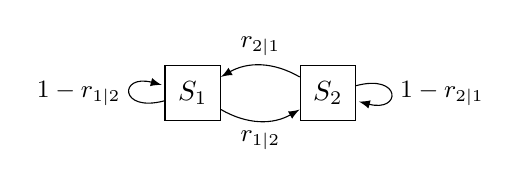
\begin{tikzpicture}[
mynode/.style={
  draw,
  minimum size=2em
  },
every loop/.append style={-latex},  
start chain=going right  
]
\foreach \Value in {1,2}
  \node[mynode,on chain] (s\Value) {$S_{\Value}$};
\path[-latex]
(s1) edge[bend right] node[auto,swap,font=\small] {$r_{1\mid2}$} (s2)
(s2) edge[bend right] node[auto,swap,font=\small] {$r_{2\mid1}$} (s1)
(s1) edge[loop left] node[left,font=\small] {$1-r_{1\mid2}$} (s1)
(s2) edge[loop right] node[right,font=\small] {$1-r_{2\mid1}$} (s2);
\end{tikzpicture}
\end{center}
with an \textit{unknown} transition matrix 
\[
\mathbf{P}=
\begin{bmatrix}
1-r_{1\mid2}&r_{1\mid2}\\
r_{2\mid1}&1-r_{2\mid1}
\end{bmatrix}
\]
where
\begin{equation}\label{eq: transition prob}
r_{i\mid j}=P[X_t=i \mid X_{t-1}=j],\quad i,j\in\{1,2\}
\end{equation}
In such scenarios, estimating the conditional probabilities $r_{i\mid j}$ is rather straightforward. Consider observing a sequence of states for individual entities at times $t-1$ and $t$. The probability of transitioning from one state to another can be estimated by calculating the ratio of the entities that transitioned from, say, $S1$ to $S2$ in the period $t-1$ to $t$ to the total number of entities that began at state $S1$ at $t-1$. In other words:
\begin{equation}\label{eq: ratio}
r_{i\mid j}=\frac{n_{ij}}{\sum_{j}n_{ij}}
\end{equation}  	  
Now, instead let us consider that the Markov chain under consideration is of order $p$ with a transition probability  
\begin{equation}\label{eq: transition prob}
r_{j_0\mid j_1,\cdots, j_p}=P[X_t=j_0 \mid X_{t-1}=j_1,\cdots,X_{t-p}=j_p],\quad j_k\in\{1,2\},\quad\text{for }k=0,1,\cdots,p
\end{equation} 
Evidently, estimating the transition probabilities is no longer trivial. In what follows, we propose methods for estimating the transition probabilities for Markov chains of high-order.   

\section{Copula-based transition matrices \label{Copula-based estimator of transition matrices}}
First, let us consider the case of a third-order stationary Markov chain with a transition matrix
\[
r_{j_0\mid j_1,\cdots,j_3}=P[X_t=j_0\mid X_{t-1}=j_1,X_{t-2}=j_2,X_{t-3}=j_3]
\]
we may express this transition matrix as

\begin{eqnarray}\label{eq: Bayes}
r_{j_0\mid j_1,\cdots,j_3}&=P[X_t=j_0,X_{t-1}=j_1,X_{t-2}=j_2\mid X_{t-3}=j_3]\bigg/P[X_{t-1}=j_1, X_{t-2}=j_2\mid X_{t-3}=j_3]
\end{eqnarray}
Furthermore, note that
\begin{align}\label{eq: radon}
\begin{split}
P[X_t=j_0,X_{t-1}=j_1,X_{t-2}=j_2\mid X_{t-3}=j_3]=&\sum\limits_{l=0,1}\sum\limits_{m=0,1}\sum\limits_{n=0,1}(-1)^{(l+m+n)}\times\\
&\mspace{-\medmuskip}P[X_t\leq j_0-l,X_{t-1}\leq j_1-m,X_{t-2}\leq j_2-n\mid X_{t-3}=j_3]
\end{split}
\end{align}
where we know from the Theorem of \citet{sklar1959fonctions} that the joint conditional distribution function on the right hand side of relationship (\ref{eq: Bayes}) can be expressed by its marginal conditional distributions and a copula function capturing their respective dependence, - i.e. 
\begin{align}\label{eq: copula}
\begin{split}
P[X_t\leq j_0-l,X_{t-1}\leq j_1-m,X_{t-2}\leq j_2-n\mid X_{t-3}=j_3]&=F(j_0-l,j_1-m, j_2-n\mid j_3)\\
&=C(F(j_0-l\mid j_3),F(j_1-m\mid j_3),F(j_2-n\mid j_3))
\end{split}
\end{align}
Therefore, using relationship (\ref{eq: copula}), we may express (\ref{eq: radon}) as follows
\begin{align}\label{eq: radoncopula}
\begin{split}
P[X_t=j_0,X_{t-1}=j_1,X_{t-2}=j_2\mid X_{t-3}=j_3]=&\sum\limits_{l=0,1}\sum\limits_{m=0,1}\sum\limits_{n=0,1}(-1)^{(l+m+n)}\times\\
&\mspace{-\medmuskip} C(F(j_0-l\mid j_3),F(j_1-m\mid j_3),F(j_2-n\mid j_3))
\end{split}
\end{align}
Therefore, the transition matrix (\ref{eq: Bayes}) can alternatively be expressed as 
\begin{equation}
r_{j_0\mid j_1,\cdots,j_3}=\frac{\sum\limits_{l=0,1}\sum\limits_{m=0,1}\sum\limits_{n=0,1}(-1)^{(l+m+n)}C(F(j_0-l\mid j_3),F(j_1-m\mid j_3),F(j_2-n\mid j_3))}{\sum\limits_{m=0,1}\sum\limits_{n=0,1}(-1)^{(m+n)}C(F(j_1-m\mid j_3),F(j_2-n\mid j_3))}
\end{equation}
In the following Proposition these results are extended to a Markov chain of order $p$.
\begin{proposition}
For a Markov chain of order $p$, the copula-based transition matrix $r_{j_0\mid j_1,\cdots, j_p}$ is expressed as follows
\begin{equation}
r_{j_0\mid j_1,\cdots,j_p}=\frac{\sum\limits_{l_0=0,1}\cdots\sum\limits_{l_p=0,1}(-1)^{(l_0+\cdots+ l_p)}C(F(j_0-l_0\mid j_p),\cdots,F(j_{p-1}-l_{p-1}\mid j_p))}{\sum\limits_{l_1=0,1}\cdots\sum\limits_{l_p=0,1}(-1)^{(l_1+\cdots+l_p)}C(F(j_1-l_1\mid j_p),\cdots,F(j_{p-1}-l_{p-1}\mid j_p))}
\end{equation} 
where $F(.\mid .)$ is a conditional distribution function and $C(u_0,\cdot,u_p)$ is a copula function in $[0,1]^{p+1}$.
\end{proposition}


\section{Estimation and inference \label{Estimation and inference}}

\subsection{Estimation \label{Estimation}}

\subsection{Inference \label{Inference}}

\section{Measuring causality in high-dimensional Markov chains \label{Measuring causality in high-dimensional Markov chains}}
\section{Monte Carlo simulations \label{Monte Carlo simulations}}

\subsection{Bootstrap bias-corrected estimator of Granger causality measures \label{Bootstrap bias-corrected estimator of Granger causality measures}}

\subsubsection{Bootstrap bias-correction \label{Bootstrap bias-correction}}

\subsubsection{Simulation study \label{Simulation study}}

\subsection{Empirical size and power \label{Empirical size and power}}

\section{Empirical application\label{Empirical application}}


\section{Conclusion \label{Conclusion}}

\newpage
\bibliographystyle{apa}
\bibliography{References_Final}

\newpage

\section{Appendix: Proofs \label{Appendix: Proofs}}
\end{document}